\documentclass{ieeeaccess}
\usepackage{cite}
\usepackage{amsmath,amssymb,amsfonts}
\usepackage{algorithm}
\usepackage{algorithmic}
\usepackage{graphicx}
\usepackage{textcomp}
\usepackage{array}
\usepackage{bm}
\makeatletter
\AtBeginDocument{\DeclareMathVersion{bold}
\SetSymbolFont{operators}{bold}{T1}{times}{b}{n}
\SetSymbolFont{NewLetters}{bold}{T1}{times}{b}{it}
\SetMathAlphabet{\mathrm}{bold}{T1}{times}{b}{n}
\SetMathAlphabet{\mathit}{bold}{T1}{times}{b}{it}
\SetMathAlphabet{\mathbf}{bold}{T1}{times}{b}{n}
\SetMathAlphabet{\mathtt}{bold}{OT1}{pcr}{b}{n}
\SetSymbolFont{symbols}{bold}{OMS}{cmsy}{b}{n}
\renewcommand\boldmath{\@nomath\boldmath\mathversion{bold}}}
\makeatother

\def\BibTeX{{\rm B\kern-.05em{\sc i\kern-.025em b}\kern-.08em
    T\kern-.1667em\lower.7ex\hbox{E}\kern-.125emX}}

\begin{document}
\history{Date of publication xxxx 00, 0000, date of current version xxxx 00, 0000.}
\doi{10.1109/ACCESS.2017.DOI}

\title{Energy Theft Probability Classification With Adaptive Observation Windows in a Digital Twin for NB-IoT Forensic Telemetry}

\author{
\uppercase{J. D. S. Coutinho Filho}\authorrefmark{1,2,4},
\uppercase{C. Marcon}\authorrefmark{3},
\uppercase{J. A. N. da Silveira}\authorrefmark{1,2},
\uppercase{R. G. Diógenes Filho}\authorrefmark{4},
AND \uppercase{M. E. Matos}\authorrefmark{5}
}

\address[1]{Department of Teleinformatics Engineering, Fortaleza, Brazil}
\address[2]{Federal University of Ceará (UFC), Fortaleza, Brazil}
\address[3]{Pontifical Catholic University of Rio Grande do Sul (PUCRS), Porto Alegre, Brazil}
\address[4]{Center of Studies and Research of the North and Northeast (NEPEN), Fortaleza, Brazil}
\address[5]{EDP South America, São José dos Campos, Brazil}

\tfootnote{This work was supported in part by the Coordenação de Aperfeiçoamento de Pessoal de Nível Superior (CAPES), Brazil, Finance Code 001, in part by the Programa de Excelência Acadêmica (PROEX), and in part by ANEEL R\&D project PD-00391-0054/25. The authors acknowledge the Núcleo de Estudos e Pesquisas do Norte e Nordeste (NEPEN), the Instituto Constanta de Inovação (ICI), and EDP South America for providing the infrastructure and material resources for this research, and acknowledge the limited use of AI-based tools for language refinement and auxiliary literature exploration during manuscript preparation. Author ORCID iDs: J. D. S. Coutinho Filho, 0009-0005-5972-7962; C. Marcon, 0000-0002-7811-7896; J. A. N. da Silveira, 0000-0003-2590-9520; R. G. Diógenes Filho, 0009-0007-5461-7937; M. E. Matos, 0009-0003-3098-3239.}

\markboth
{Coutinho Filho \headeretal: Energy Theft Probability Classification With Adaptive Observation Windows in a Digital Twin for NB-IoT Forensic Telemetry}
{Coutinho Filho \headeretal: Energy Theft Probability Classification With Adaptive Observation Windows in a Digital Twin for NB-IoT Forensic Telemetry}

\corresp{Corresponding author: J. D. S. Coutinho Filho (e-mail: danilocoutinho@lesc.ufc.br).}

\begin{abstract}
Non-technical losses remain a major challenge for electric power distribution utilities because suspicious consumption behavior is often intermittent, which makes fixed-cadence telemetry either insufficient for forensic analysis or wasteful of communication resources. This paper presents a digital-twin-driven framework that treats telemetry density as a controllable resource, adapting the observation window of a dedicated forensic metering device according to contextual theft-risk estimation. The framework fuses forensic and billing measurements, derives contextual and temporal features, and combines a rule-based and a supervised risk engine through three probability-fusion strategies. An orchestration layer converts the fused risk into a discrete observation-mode decision, and a communication-cost model grounded in reported narrowband Internet of Things (NB-IoT) quality-of-service measurements accounts for signaling overhead, retransmission, and latency. The resulting detection-versus-communication-cost trade-off is resolved empirically through a Pareto-frontier analysis over the fusion weight and the decision thresholds, and a computational-scalability benchmark verifies that per-device processing cost does not grow with fleet size. Experiments across seven controlled synthetic scenarios, including heterogeneous fraud severities and degraded-link conditions, show that the adaptive policy retains about 91\% of the F1-score and 83\% of the recall of dense, native-resolution monitoring while transmitting only about 30\% of the communication volume. These results indicate that digital twins can act as application-aware sensing controllers, and not only as passive monitors, in communication-constrained smart-metering deployments.
\end{abstract}

\begin{keywords}
Adaptive telemetry, closed-loop optimization, digital twin, energy theft detection, narrowband Internet of Things, non-technical losses, Pareto optimization.
\end{keywords}

\titlepgskip=-21pt

\maketitle

\section{Introduction}
\label{sec:introduction}
\PARstart{N}{on-technical} losses (NTLs) remain a significant challenge for power distribution utilities, regulators, and sector operators. Among their most recurrent causes are energy theft, partial or selective bypass, meter tampering, and other fraudulent consumption mechanisms that directly affect revenue collection and the reliability of operational supervision. In practice, such behaviors tend to occur at specific times of day or under particular operating conditions, rather than continuously, and utilities report that the diverted fraction of consumption itself varies with the fraud strategy adopted, from constant partial diversion to brief, near-total diversion confined to specific hours. This temporal and behavioral heterogeneity makes conventional fixed-period monitoring strategies intrinsically limited for forensic purposes.

At low acquisition rates, relevant evidence may not be captured when suspicious behavior occurs, whereas maintaining permanently high sampling and transmission rates imposes communication costs disproportionate to the operational benefit during normal operation. Thus, the central challenge is not only to classify theft risk from telemetry, but also to determine when increasing the temporal resolution of observation is technically justified, and to do so under communication conditions that are representative of the target radio technology rather than an abstract cost proxy.

Although the literature on NTL detection has reported increasingly robust classification results using smart meter and Advanced Metering Infrastructure (AMI) data, most approaches inherently assume fixed-cadence measurement streams and focus on improving classification within a predefined observation process \cite{b2,b4,b5,b6}. In parallel, digital-twin studies for smart metering have predominantly emphasized virtualization and monitoring, rather than application-oriented control of the sensing process \cite{b19,b20,b22}. Similarly, adaptive telemetry methods in IoT and low-power wide-area network (LPWAN) systems have largely focused on bandwidth or energy efficiency, without explicitly linking sensing density to the forensic value of the observed context \cite{b26,b27,b29}. As a result, an important gap remains at the intersection of these research lines: the lack of a closed-loop framework in which a digital twin integrates contextual evidence and dynamically adapts observation density based on its expected forensic utility, while being evaluated against a realistic, heterogeneous fraud population and a network-representative communication-cost model. This gap motivates the central hypothesis of this work: an application-oriented digital twin can use contextual theft-risk estimates to adapt the observation window of NB-IoT forensic telemetry, thereby preserving most of the detection performance associated with dense monitoring while substantially reducing communication cost, and this trade-off can be characterized and resolved explicitly rather than left implicit. Under this formulation, risk estimation is treated as a control signal that governs the observation process, reframing the problem from static classification toward application-oriented closed-loop optimization.

In this work, the digital twin is defined as an application-oriented software entity that maintains contextual state, integrates heterogeneous measurements, estimates the probability of theft, and feeds the result back into the telemetry-configuration process. Section~\ref{subsec:twin_criteria} makes this definition operational by mapping four established digital-twin criteria (state persistence, bidirectional synchronization with a physical asset, closed-loop decision-making, and use as an active control layer rather than a passive monitor) to the specific software components implemented in this study, and states explicitly which of these criteria are satisfied in a physically closed loop today and which remain closed only in simulation. In this sense, the twin acts as a decision layer that converts contextual evidence into sensing actions, consistent with the broader view of digital twins as closed-loop cyber-physical mechanisms for monitoring, prediction, and adaptive control \cite{b15,b16,b24}.

The system considered in this paper consists of a dedicated forensic telemetry device installed in parallel with the billing meter, using NB-IoT as the primary communication technology and Bluetooth Low Energy (BLE) as a local contingency channel. The forensic device is a discrete, already-implemented and certified embedded product (conducted and radiated immunity per IEC 61000-4-4, IEC 61000-4-5, IEC 61000-4-6, and IEC 61000-4-11) with a metrological error class equivalent to the billing meter it monitors; its firmware-level design is outside the scope of the present study, whose contribution lies entirely in the software layer of the digital twin that combines billing and inspection measurements, derives contextual features, estimates the probability of theft, and governs a closed-loop adaptive observation-window policy. The device is powered from the distribution network itself and is therefore available full-time; consequently, this study does not model device energy consumption as a constraint, and instead targets the utility's primary operational concern for this class of system: minimizing the volume and cost of transmitted forensic data without compromising detection capability.

Fig.~\ref{fig:use_case_topology} summarizes the physical and logical topology considered in this work, highlighting the placement of the inspection meter on the utility service branch, its relationship to the billing meter, and the telemetry flow toward the analytics platform.

\begin{figure}[t]
    \centering
    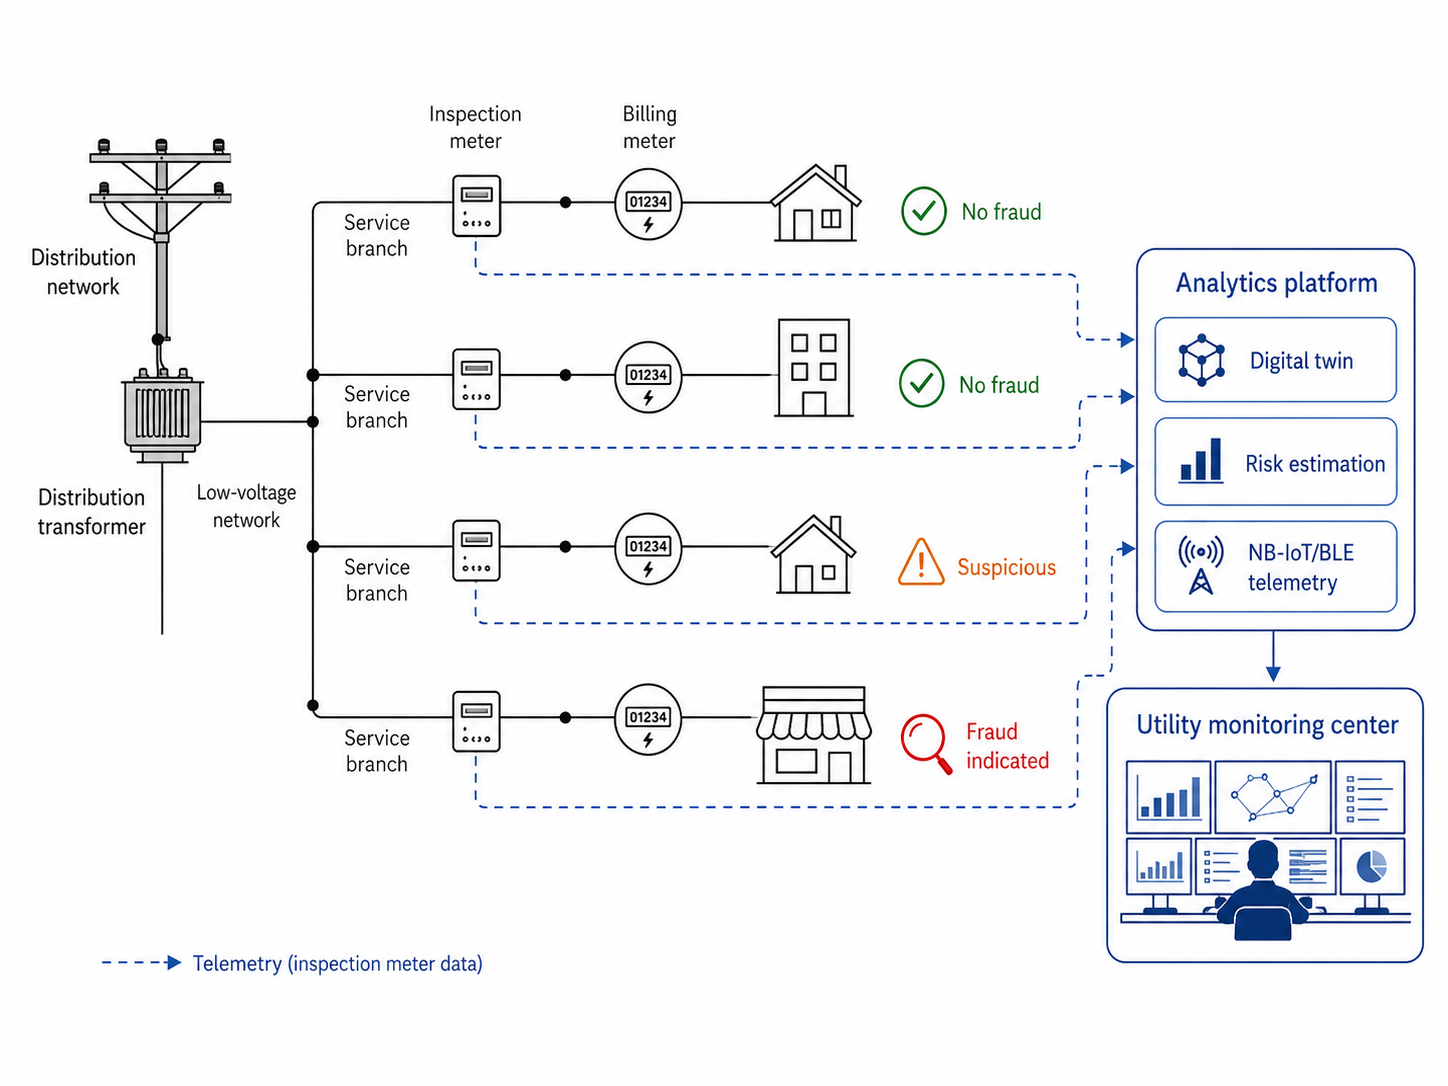
\includegraphics[width=\columnwidth]{fig/topologia_artigo.png}
    \caption{Simplified use-case topology of the proposed forensic telemetry framework.}
    \label{fig:use_case_topology}
\end{figure}

The main contributions of this work are sixfold:
\begin{itemize}
    \item formulating energy-theft monitoring as a closed-loop observation-control problem, in which telemetry density is treated as a controllable resource, with detection capability and communication cost formalized as explicit functions of the twin's observational state and the selected observation action;
    \item designing and implementing an application-oriented digital twin for forensic energy telemetry that fuses billing and inspection data into contextual theft-risk estimates, and stating explicitly which established digital-twin criteria the implementation satisfies at its current stage of integration;
    \item generating synthetic experimental data with heterogeneous fraud severities and profiles, independent measurement and communication noise, and a native acquisition resolution fine enough to make every observation mode operationally distinguishable, so that the resulting classification problem is not an artifact of the data-generation process;
    \item proposing an adaptive observation-window policy and empirically resolving its detection-versus-communication-cost trade-off through a Pareto-frontier analysis over the fusion weight and decision thresholds, rather than leaving these parameters as unjustified constants;
    \item modeling the NB-IoT/Bluetooth Low Energy communication cost with signaling overhead, retransmission, and latency grounded in reported quality-of-service measurements, evaluated consistently across every observation policy considered; and
    \item providing a fully reproducible seven-scenario experimental campaign, complemented by a feature-importance analysis, an alternative-model comparison, and a computational-scalability benchmark, for a controlled comparison between fixed and adaptive observation policies under both detection and communication-cost metrics.
\end{itemize}

The remainder of this paper is organized as follows. Section~\ref{sec:related_work} situates the work within the literature and makes explicit the research gap it addresses. Section~\ref{sec:system_model} presents the system model and the formal problem statement. Section~\ref{sec:Materials_Methods} describes the proposed framework, including the reproducible prototype architecture, the digital-twin scope, the synthetic-data methodology, the risk and fusion engines, the communication-cost model, and the complexity analysis. Section~\ref{sec:Results_Discussion} presents and discusses the results, including a critical assessment of limitations. Section~\ref{sec:Conclusion} concludes the paper.

\section{Related Work}
\label{sec:related_work}
This section reviews the most relevant literature related to the problem addressed in this paper, focusing on three axes: (i) energy theft and NTL detection in smart metering, (ii) the use of digital twins in smart metering and cyber-physical monitoring, and (iii) adaptive telemetry under communication constraints. Rather than providing a purely descriptive overview, this section aims to situate the present work relative to the closest studies and to clarify which capabilities are already available in the literature and which combinations remain insufficiently explored.

\subsection{Bibliographic Search Strategy and Study Selection}
The related literature was identified through a structured search in major databases (IEEE Xplore, Springer, ScienceDirect, and MDPI), covering publications from 2019 to 2025, with updates through March 2026. The search strategy was designed to cover the three central components of the problem investigated in this paper: energy-theft detection, digital-twin-based monitoring, and adaptive telemetry.

The search was guided by the following three complementary queries:
\begin{itemize}
    \item \textit{\textbf{Query A --- Energy theft and non-technical-loss detection:} (``energy theft" OR ``electricity theft" OR ``non-technical loss*" OR NTL OR fraud OR tamper*) AND (``smart meter*" OR ``advanced metering infrastructure" OR AMI) AND (detect* OR classif* OR anomal* OR ``machine learning" OR ``deep learning")}
    \item \textit{\textbf{Query B --- Digital twins for smart metering and energy monitoring:} (``digital twin*" OR ``cyber-physical" OR ``virtual replica") AND (``smart meter*" OR ``smart grid" OR ``power distribution" OR ``energy monitoring") AND (monitor* OR anomaly OR fault OR secur* OR telemetry OR ``real-time")}
    \item \textit{\textbf{Query C --- Adaptive telemetry and communication-efficient monitoring:} (("NB-IoT" OR "narrowband IoT" OR LPWAN OR BLE OR telemetry OR "remote metering") AND ("smart meter*" OR "energy meter*" OR "forensic telemetry") AND (adaptive OR dynamic OR "observation window*" OR "sampling rate" OR "transmission interval" OR reconfigur* OR "closed-loop"))}
\end{itemize}

The queries were applied, with minor syntactic adaptations, across the different bibliographic databases. The initial retrieval yielded 91 records. After duplicate removal, 78 records remained. Screening by title, abstract, and keywords reduced this set to 42 studies; full-text review yielded a final core set of 31 works discussed in this section, complemented by a small, targeted set of additional references introduced in Sections~\ref{sec:system_model} and~\ref{sec:Materials_Methods} to ground the communication-cost model and the relaxed temporal-evaluation metric in measurement-based and methodological literature, respectively.

As inclusion criteria, studies were retained if they presented at least one of the following aspects: (i) methods for energy-theft or non-technical-loss detection using smart meter or AMI data; (ii) digital-twin-based approaches for smart metering, smart grids, or energy monitoring; or (iii) adaptive telemetry, sensing, or communication strategies relevant to NB-IoT, LPWAN, or resource-constrained IoT monitoring. Exclusion criteria removed generic works on IoT, smart cities, or digital twins that had no direct relation to smart metering, energy monitoring, or adaptive observation, as well as studies whose contributions were distant from the forensic telemetry problem addressed in this paper.

Rather than being a full systematic review, this procedure should be interpreted as a structured, reproducible bibliographic selection protocol aimed at technically positioning the present study. The resulting corpus was organized into three groups corresponding to the main research lines discussed next.

\subsection{Energy-Theft and Non-Technical-Loss Detection from Smart Metering Data}
The detection of NTLs and the identification of energy theft have been extensively investigated using data collected from smart meters and AMI. Previous studies have shown that supervised machine learning, deep learning, and ensemble-based methods can detect suspicious consumption behavior with good classification performance when historical load series are available \cite{b1, b2, b3, b4, b5, b6}.

This body of literature has evolved from conventional classifiers to more sophisticated architectures designed to address class imbalance, temporal variation, and attack diversity. CNN-based, CNN-LSTM, transformer-based, and stacked-ensemble models have been proposed to improve discrimination between legitimate and malicious users, while one-class and zero-day approaches seek to generalize to previously unseen fraud patterns \cite{b7, b8, b9, b10, b11, b12}. More recently, reinforcement learning has also been explored to detect theft cyberattacks and adapt to evolving consumption patterns and newly launched attack strategies \cite{b38}, which reinforces, from a detection-model perspective, the same behavioral heterogeneity that motivates the fraud-profile modeling adopted in Section~\ref{subsec:synthetic_realism} of this paper. Other studies have incorporated clustering strategies, feeder-level aggregation, or contextual customer modeling to reduce false positives and increase robustness to heterogeneous consumption profiles \cite{b13, b14}.

Despite these advances, the dominant assumption in most NTL studies is that telemetry is already available at a fixed cadence. As a consequence, prior work has focused on improving classification under a predefined observation process, rather than questioning whether the observation process itself should be dynamically adapted to the forensic relevance of the current context \cite{b2, b5, b6}.

\subsection{Digital Twins for Smart Metering and Cyber-Physical Monitoring}
In parallel with research on energy-theft detection, digital twins have emerged as an important paradigm for cyber-physical monitoring, prediction, and decision support. In general terms, a digital twin maintains a synchronized virtual representation of a physical asset or process and exploits this representation for monitoring, fault analysis, simulation, and operational guidance \cite{b15, b16, b17}. In energy-related domains, digital twins have been applied to smart-meter virtualization, real-time monitoring, predictive analysis, communication-aware services, and secure integration of IoT-based systems \cite{b18, b19, b20, b21, b22}.

In the context of smart metering, existing digital-twin studies emphasize the virtualization of meter functions, bidirectional communication between the device and the cloud, and the use of real-time monitoring dashboards that support operational services and remote interaction \cite{b19, b20, b22}. More broadly, the digital-twin literature highlights closed-loop monitoring, predictive maintenance, and adaptive control as central properties of mature cyber-physical deployments \cite{b23, b24, b25}. However, in smart metering, the twin is still used predominantly for representation, supervision, and service support, rather than as an application-oriented decision layer that can reallocate sensing effort based on contextual value \cite{b18, b20, b22}. This limits the role of digital twins to passive monitoring, leaving unexplored their potential as active sensing and control entities.

\subsection{Adaptive Telemetry and the Still-Unresolved Intersection}
A third body of literature addresses adaptive telemetry, communication-efficient monitoring, and anomaly detection in IoT and industrial systems. These studies show that dynamic transmission policies, adaptive anomaly detection, and edge-assisted intelligence can reduce bandwidth or energy consumption while preserving monitoring capability \cite{b26, b27, b28}. In smart-metering and LPWAN scenarios, adaptive algorithms have also been proposed to adjust transmission intervals based on the observed dynamics of sensed data, yielding significant savings in packet volume and communication-related energy costs, including in NB-IoT environments \cite{b29}. Related NB-IoT smart-metering work also reinforces the feasibility of lightweight, long-range telemetry for remote measurement and distributed configuration \cite{b30, b31}, and field- and simulation-based quality-of-service characterizations of commercial NB-IoT deployments provide concrete latency, coverage, and signaling-overhead figures that this paper uses directly to parameterize its communication-cost model rather than treating communication volume as an abstract proxy (see Section~\ref{subsec:network_cost}) \cite{b32,b33,b34,b35}.

These adaptive-telemetry studies usually optimize communication efficiency for generic monitoring objectives rather than for application-oriented tasks such as distinguishing theft from non-theft conditions. In contrast, energy-theft detection studies typically optimize classification accuracy while assuming a fixed observation process, whereas digital-twin studies in smart metering rarely turn observation density itself into a decision-controlled variable. This leaves open the combination of contextual theft-risk estimation, digital-twin-based decision support, and adaptive observation under communication constraints \cite{b6, b14, b22, b29}.

The present study is positioned at this intersection. Rather than treating telemetry cadence as fixed, it models sensing density as a controllable resource and uses the digital twin as a closed-loop decision layer for risk-driven forensic observability in LPWAN-based telemetry, specifically using NB-IoT.

\subsection{Comparative Summary}

\begin{table*}[!ht]
\centering
\caption{Positioning of this work relative to the closest literature}
\label{tab:rw_comparison}
\begin{tabular}{|p{2cm}|p{4.6cm}|p{2.4cm}|p{4.1cm}|p{1.9cm}|}
\hline
\textbf{Research line} & \textbf{Core contribution} & \textbf{Typical assumption} & \textbf{Main limitation} & \textbf{Representative references} \\
\hline
Energy theft / NTL detection & Theft detection from smart meter or AMI data using ML, DL, ensembles, or anomaly models & Fixed-cadence telemetry & Does not treat observation density as a control variable & \cite{b1,b2,b3,b4,b5,b6,b7,b8,b9,b10,b11,b12,b13,b14,b38} \\
\hline
Digital twins for smart metering & Virtualization, synchronized monitoring, remote interaction, and operational support & Twin used mainly for supervision or services & Rarely uses the twin as an application-aware sensing control layer & \cite{b18,b19,b20,b21,b22,b23,b24,b25} \\
\hline
Adaptive telemetry / communication-efficient monitoring & Dynamic reporting for bandwidth or energy reduction; NB-IoT quality-of-service characterization & Efficiency-driven adaptation; communication cost as bytes or energy & Does not optimize telemetry for theft-oriented forensic utility & \cite{b26,b27,b28,b29,b30,b31,b32,b33,b34,b35} \\
\hline
This work & Contextual theft-risk estimation with digital-twin-guided adaptive observation for NB-IoT forensic telemetry, with an explicit, measurement-grounded cost model and an empirically resolved cost-detection trade-off & Observation density is controllable & Balances detection capability and communication cost; validated on synthetic data pending field-data disclosure & This article \\
\hline
\end{tabular}
\end{table*}

Table~\ref{tab:rw_comparison} summarizes the positioning of the present work with respect to the three closest lines of literature. In summary, prior literature provides important foundations in three complementary directions: energy-theft detection from smart meter data, the use of digital twins for monitoring and decision support, and adaptive telemetry in communication-constrained IoT systems. However, these components remain only weakly articulated in the context of forensic observability in electrical metering systems. The main gap, therefore, is the lack of frameworks that explicitly treat observation density as a controllable resource, leverage digital twins as decision layers to allocate sensing effort based on contextual forensic value, and resolve the resulting cost-detection trade-off explicitly rather than through unjustified fixed parameters.

\section{System Model and Problem Formulation}
\label{sec:system_model}
The problem investigated in this work is formulated as an adaptive observation-control problem in forensic telemetry. At each potential acquisition instant $t$, the system has access to an observational state $s_t$ summarizing the electrical, temporal, operational, and historical conditions of the monitored asset. In the current prototype, $s_t$ includes, among other variables, relative power divergence, accumulated energy difference, moving averages of divergence over real-time windows, hourly recurrence, alarm score, and the operational-integrity signals \textit{link} and \textit{heartbeat}. Based on $s_t$, the digital twin selects an action $a_t \in \mathcal{A} = \{\text{basal},\, \text{moderate},\, \text{aggressive}\}$, where each action induces a distinct capture interval $\Delta(a_t) \in \{60, 15, 5\}$ minutes, respectively.

The system dynamics are partially controlled: the action taken at time $t$ alters the future observation density, which changes the information available at subsequent times. This distinguishes the problem from static classification over a fixed sample set, since the decision policy affects the observation process that will feed future decisions.

Let $o_t(a_{1:t}) \in \{0,1\}$ denote whether the forensic device emits (is observed) at instant $t$ under the capture schedule induced by the action history up to $t$ (Algorithm~\ref{alg:closed_loop_twin}), and let $p_t^{(d)}(s_t) \in [0,1]$ denote the fused decision probability produced by the twin (Section~\ref{subsec:fusao}). Let $y_t \in \{0,1\}$ denote the (unobserved, ground-truth) theft-activity indicator and $\tau$ the decision threshold. The detection capability of a policy over a horizon of $T$ instants is defined as
\begin{equation}
D\big(s_{1:T}, a_{1:T}\big) = \frac{1}{\sum_{t=1}^{T} y_t} \sum_{t=1}^{T} y_t \cdot o_t(a_{1:t}) \cdot \mathbb{1}\!\left[p_t^{(d)}(s_t) \geq \tau\right],
\label{eq:detection_capability}
\end{equation}
that is, the fraction of ground-truth theft instants that are both observed and correctly flagged; this is precisely the recall of the induced policy, made explicit here as a function of the state trajectory (through $p_t^{(d)}$) and the action trajectory (through $o_t$). Let $b_t(s_t)$ denote the per-event communication cost in bytes returned by the transport-cost model of Section~\ref{subsec:network_cost}, which depends on the operational context captured in $s_t$ (link and heartbeat state) and on whether a fresh NB-IoT connection must be established. The communication cost of a policy is
\begin{equation}
C\big(s_{1:T}, a_{1:T}\big) = \sum_{t=1}^{T} o_t(a_{1:t}) \cdot b_t(s_t).
\label{eq:communication_cost}
\end{equation}
The objective of the digital twin is to select an action sequence that maximizes
\begin{equation}
U\big(a_{1:T}\big) = \lambda_1 \cdot D\big(s_{1:T}, a_{1:T}\big) - \lambda_2 \cdot C\big(s_{1:T}, a_{1:T}\big),
\label{eq:utility}
\end{equation}
where $\lambda_1, \lambda_2 \geq 0$ express the relative importance of forensic sensitivity and communication efficiency. Searching directly over the space of action sequences is combinatorial ($|\mathcal{A}|^T$) and requires committing to a specific $(\lambda_1, \lambda_2)$ pair a priori. Section~\ref{subsec:pareto} instead restricts the search to a low-dimensional, interpretable policy-parameter family $\Theta = (\alpha, \tau_{\text{moderate}}, \tau_{\text{high}})$, comprising the fusion weight (Section~\ref{subsec:fusao}) and the two hysteresis thresholds that fully determine the induced action sequence given an observation trace, and empirically traces the Pareto-optimal frontier of $\big(D(\Theta), C(\Theta)\big)$ over a grid of $\Theta$. Because the Pareto frontier is, by construction, the set of policies that are optimal for \emph{some} non-negative $(\lambda_1, \lambda_2)$, this sidesteps the need to fix the exchange rate between detection and cost a priori: a decision-maker can select any operating point on the frontier according to the locally implied $\lambda_1/\lambda_2$ ratio (the frontier's slope at that point), and the configuration used elsewhere in this paper is reported explicitly as either on or near this empirical frontier (Section~\ref{subsec:results_pareto}), rather than as an unjustified constant.

Since Eq.~\eqref{eq:utility} is not directly observable during deployment, the experimental evaluation approximates $D$ and $C$ using precision, recall, F1-score, and a critical-slot metric for the detection side, and communication bytes, latency, and retransmission counts for the cost side (Section~\ref{subsec:metrics}). Under this formulation, the problem solved by the framework is not merely to classify theft versus non-theft, but to decide when it is worthwhile to increase the temporal resolution of observation, with the risk probability estimated by the twin's engines acting as the control signal that governs telemetry density.

\section{Materials and Methods}
\label{sec:Materials_Methods}
\subsection{Methodological Overview}
This section describes the experimental framework implemented to evaluate energy-theft probability classification with adaptive observation control in an NB-IoT-based forensic telemetry scenario. The methodological objective is not merely to estimate risk from previously available telemetry, but to materialize an application-oriented digital twin capable of interpreting context, determining observation density, and locally updating the capture regime throughout the experimental execution.

The framework was built as a reproducible local-execution prototype, fully implemented in Python, with simplified installation, SQLite persistence, and command-line execution. This design choice had two main motivations. First, it ensured that the experiments reported in the paper could be reproduced without mandatory dependence on external infrastructure. Second, it allowed the digital-twin architecture to be made explicit in code before integration with real data, an NB-IoT broker, and real-time BLE contingency.

Conceptually, the framework is organized into seven layers: data ingestion, contextual enrichment, risk engines, explicit digital-twin state, policy orchestration, a local closed-loop runtime with simulated devices, and a communication-cost/complexity evaluation layer. Unlike a static classification pipeline, the current implementation contains explicit entities for twin state, decision, command plan, transport cost, and execution of the perception-decision-action cycle.

\subsection{System Under Consideration and Firmware-Integration Assumptions}
The target system consists of a billing meter and a discrete forensic telemetry device installed in parallel with the monitored installation. The forensic device is an already-implemented, certified embedded product, compliant with the electromagnetic-compatibility immunity requirements of IEC 61000-4-4 (electrical fast transient/burst), IEC 61000-4-5 (surge), IEC 61000-4-6 (conducted radio-frequency disturbances), and IEC 61000-4-11 (voltage dips, short interruptions, and variations), and engineered with a metrological error class equivalent to that of the billing meter it monitors, so that forensic-versus-billing divergence reflects a genuine metering discrepancy rather than an artifact of instrument-class mismatch. The device is intentionally discreet, so that its presence is not readily apparent to the customer whose installation is being inspected. It is assumed that the embedded layer already provides instantaneous electrical quantities, historical profiles, alarms, local persistence, and telemetry parameters remotely configurable via NB-IoT, with BLE available as a local contingency channel. The device is powered from the monitored installation's own network connection and is therefore available full-time; device energy consumption is consequently outside the scope of this study; the operational cost that matters to the distribution utility, and that this paper targets, is the volume and cost of transmitted data.

At this stage of the study, integration with the physical layer is represented by synthetic traces semantically aligned with the firmware domain. The field names used in data generation and processing preserve this semantic proximity without breaking the logical architecture of the framework: the electrical quantities follow the instantaneous-metrology naming used by the firmware (e.g., \texttt{voltage\_rms}, \texttt{active\_power}, \texttt{power\_factor}), and the alarm flags follow the firmware's alarm-manager naming (e.g., \texttt{alarm\_overvoltage}, \texttt{alarm\_overcurrent}).

\subsection{Digital-Twin Criteria and Scope}
\label{subsec:twin_criteria}
Because the term ``digital twin'' is used inconsistently across the literature, this subsection makes explicit which criteria the implementation satisfies, and to what degree, rather than asserting the label without justification. Following the broader cyber-physical-systems view of digital twins as closed-loop mechanisms for monitoring, prediction, and control \cite{b15,b16,b24}, four criteria are considered:

\begin{enumerate}
    \item \textit{State persistence.} The \textit{ForensicTwin} entity maintains an explicit, event-indexed state (current observation mode, capture period, mode-dwell count, last decision probabilities, and last command) that is snapshotted and persisted at every observed event, independent of any single classification call. This criterion is fully satisfied by the current implementation.
    \item \textit{Bidirectional synchronization with a physical asset.} The twin both receives evidence from, and issues reconfiguration commands to, the forensic device's emission schedule. In the present study, this synchronization loop is materialized with a locally simulated device (\textit{MockForensicDevice}) and transport (\textit{MockTransport}), because the physical forensic device described in Section~\ref{sec:Materials_Methods}.B already exists and is certified, but end-to-end NB-IoT/BLE integration with the twin software is planned future work. This criterion is therefore satisfied at the software-architecture level and in a local closed loop, but not yet validated against a physically deployed radio link.
    \item \textit{Closed-loop decision-making.} The action selected at time $t$ (Section~\ref{sec:system_model}) changes the future observation density, which changes the evidence available to subsequent decisions. Algorithm~\ref{alg:closed_loop_twin} and the runtime evidence reported in Section~\ref{sec:Results_Discussion} (distinct sample counts per observation mode, issued reconfiguration commands, transport-delivery records) demonstrate that this loop is exercised, not merely described. This criterion is fully satisfied within the local runtime.
    \item \textit{Active sensing/control layer, not a passive monitor.} Unlike the smart-metering digital-twin studies discussed in Section~\ref{sec:related_work}, which use the twin primarily for virtualization, dashboards, and supervision \cite{b18,b19,b20,b22}, the twin in this work is the entity that decides the telemetry density itself. This is the paper's central architectural claim and is fully satisfied by construction.
\end{enumerate}

In summary, this study implements the software layer of an application-oriented digital twin, with three of the four criteria fully realized in a physically closed loop and the fourth (physical bidirectional synchronization) currently closed only in a local, reproducible simulation rather than over a deployed radio link. This scoping is stated explicitly rather than left implicit, and is treated further as a threat to validity in Section~\ref{subsec:limitations}.

\subsection{Implemented Digital-Twin Architecture}
The core of the framework is the \textit{ForensicTwin} digital twin, implemented as a software entity with its own state and event-oriented updates. At each observed event, the twin receives a \textit{TwinObservation}, produced from the temporal fusion of forensic measurements, billing measurements, and alarm events. This observation contains the electrical, temporal, operational, and alarm-related attributes required for risk inference.

A \textit{DecisionEngine} operates on this observational state and is responsible for transforming the current context into a probabilistic risk decision. The engine uses two evidence sources: a rule-based contextual baseline and a supervised logistic-regression baseline. Rather than assuming a single fixed combination rule, the framework supports three explicit probability-fusion strategies: \textit{weighted}, \textit{conservative\_max}, and \textit{context\_aware} (Section~\ref{subsec:fusao}).

The output of the \textit{DecisionEngine} is consumed by a \textit{PolicyOrchestrator}, which converts the decision into an observational action. This action is formalized in the \textit{TelemetryReconfigurationDecision} structure, which represents the command plan issued by the digital twin. Among other fields, the command specifies the monitored asset identifier, the selected mode, the capture interval, the decision probability, the probability source, the textual justification, and the preferred transport.

To materialize the closed loop in a local environment, the framework further uses three simulation components: \textit{MockForensicDevice}, \textit{MockBillingMeter}, and \textit{MockTransport}. The first simulates the forensic device and adjusts its future emission cadence based on the received command. The second provides the billing reference. The third simulates local command delivery, with preferential use of NB-IoT and fallback to BLE in degraded scenarios (which, in a real system, would require a local operator with a BLE-enabled device), using the communication-cost model of Section~\ref{subsec:network_cost}. The integrated execution of these components is handled by \textit{SimulationRunner}, which explicitly implements the framework's local closed loop.

\begin{figure*}[!t]
      \centering
      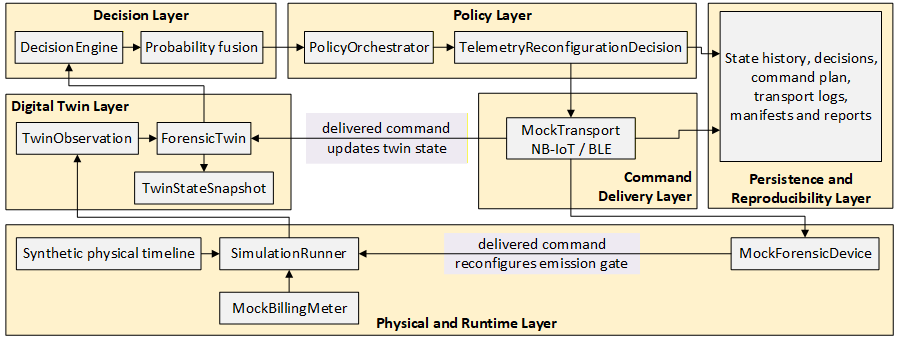
\includegraphics[width=0.9\textwidth]{fig/framework_architecture2.png}
      \caption{Closed-loop architecture of the proposed digital-twin framework.}
      \label{fig:framework_architecture}
\end{figure*}

The implemented framework architecture is summarized in Fig.~\ref{fig:framework_architecture}. As shown, the core of the system is composed of the \textit{ForensicTwin}, the decision layer \textit{DecisionEngine}, the policy-orchestration layer \textit{PolicyOrchestrator}, and the explicit command-plan formalization \textit{TelemetryReconfigurationDecision}. These components operate jointly with the local runtime and the simulated devices, materializing a closed loop in which the twin's decision changes the future observation density.

\subsection{Formalization of the Local Closed Loop}
The local runtime executes the following cycle in temporal order:
\begin{enumerate}
    \item traverses the synthetic physical timeline at native resolution;
    \item checks, through the \textit{MockForensicDevice}, whether the current event should be emitted according to the active capture interval;
    \item whenever the event is emitted, constructs a \textit{TwinObservation};
    \item evaluates the observation with the \textit{DecisionEngine};
    \item applies a probabilistic fusion strategy;
    \item generates a \textit{TelemetryReconfigurationDecision} with the \textit{PolicyOrchestrator};
    \item delivers the command through the \textit{MockTransport}, which resolves NB-IoT/BLE selection and the resulting cost/latency;
    \item applies the command to the \textit{ForensicTwin} and to the \textit{MockForensicDevice}; and
    \item updates the twin state and the future emission cadence.
\end{enumerate}

\begin{algorithm}[!ht]
\caption{Local closed loop of the digital twin}
\label{alg:closed_loop_twin}
\begin{algorithmic}[1]
\REQUIRE Synthetic timeline $\mathcal{X}$, twin $T$, forensic device $D$, billing meter $B$, transport $L$
\FORALL{instant $x_t \in \mathcal{X}$}
    \IF{$D.\text{should\_emit}(x_t)$}
        \STATE $o_t \gets \text{build\_observation}(x_t, B)$
        \STATE $d_t \gets T.\text{update}(o_t)$
        \STATE $c_t \gets \text{PolicyOrchestrator}(d_t)$
        \STATE $L.\text{deliver}(c_t)$
        \STATE $T.\text{apply}(c_t)$
        \STATE $D.\text{apply}(c_t)$
    \ENDIF
\ENDFOR
\end{algorithmic}
\end{algorithm}

This modeling choice is important because it shifts the experiment from a simple offline evaluation on fixed samples to an environment in which observability itself becomes a consequence of the twin's decisions. Although the physical loop is local and simulated, the logical structure of perception, inference, action, and feedback is already explicitly materialized, and its runtime cost is characterized in Section~\ref{subsec:complexity}.

\subsection{Native Temporal Resolution and Observation Modes}
\label{subsec:native_resolution}
The native acquisition grid of the synthetic physical timeline is set to 5 minutes, an exact common divisor of the three observation-mode capture periods used by the policy orchestrator: \textit{basal} (60 minutes), \textit{moderate} (15 minutes), and \textit{aggressive} (5 minutes). This choice is methodologically necessary: the forensic-device emission gate (Algorithm~\ref{alg:closed_loop_twin}, line 2) can never emit faster than data exists on the underlying timeline, so a native resolution coarser than the finest observation mode would make that mode indistinguishable, at the data level, from any mode with an equal or coarser capture period. With the 5-minute native grid, \textit{aggressive} observes every native tick, \textit{moderate} observes every third tick, and \textit{basal} observes every twelfth tick, so the three modes induce genuinely different observation densities; this property is verified directly by a unit test that drives the device emission gate over a synthetic 5-minute-spaced timeline and asserts the expected 12:4:1 emission ratio across aggressive, moderate, and basal modes.

A direct consequence of this resolution choice is that a fixed policy reporting on a 15-minute cadence (\textit{fixed\_short}, retained from earlier campaigns as an intermediate, realistic fixed-cadence baseline) is a genuinely sparser policy than the native acquisition grid, and can therefore no longer serve as a proxy for "dense monitoring." Accordingly, this study introduces a fourth policy, \textit{fixed\_dense}, which reports at the native 5-minute resolution and is used throughout Section~\ref{sec:Results_Discussion} as the empirical ceiling against which the detection performance of every other policy, fixed or adaptive, is compared.

\subsection{Synthetic Data Generation: Metrological Coherence, Realistic Noise, and Heterogeneous Fraud Profiles}
\label{subsec:synthetic_realism}
The experimental campaign is built upon seven controlled synthetic scenarios: normal operation, persistent theft, peak-hour theft, nighttime theft, intermittent nighttime theft, disturbance without theft, and a degraded-link scenario without theft. Each scenario covers seven days of observation at the native 5-minute resolution. Generation is deterministic, with explicit random seeds, producing three temporal streams per scenario: forensic-device measurements, billing-meter measurements, and alarm events.

The synthetic traces preserve metrological coherence among voltage, current, active power, reactive power, apparent power, power factor, and accumulated energies: at each interval, RMS voltage and active power are first defined from the scenario load profile, after which the power factor is sampled within a plausible range and used to consistently derive apparent power, reactive power, and RMS current; active and reactive energies are then accumulated over time according to the native time step. This ensures that the risk features extracted by the framework correspond to electrically plausible observational discrepancies rather than to arbitrary differences between artificial time series.

Two properties of the data-generation process are essential to the internal validity of the classification problem addressed in this paper, and are made explicit here because they directly determine whether the reported detection metrics are meaningful or an artifact of how the labels were produced. First, the discrepancy between the forensic and billing readings is not treated as a single deterministic function of a scenario-level theft ratio. Independent, theft-unrelated noise sources are added to both meters: per-meter metrological noise (approximately 1.2\% relative standard deviation, applied independently to the forensic and billing active-power readings before the internally consistent electrical quantities are derived), transient communication/reporting glitches (occurring with 3\% per-tick probability, at a magnitude comparable to a low-severity theft event, and applied at random to either meter), and legitimate but erratic load surges (occurring with 1.5\% per-tick probability, representing events such as a large appliance motor start) that are independent of theft activity. The out-of-bounds-power alarm, which in an earlier version of this framework was derived directly from the forensic-versus-billing gap, is redefined here using only the forensic meter's own reading against a fixed contracted-demand ceiling, so that no alarm used as a classification feature can, by construction, encode the detection label.

Second, theft severity and temporal behavior are made heterogeneous rather than uniform, reflecting the diversity of fraud strategies reported in practice, from constant partial diversion to brief, near-total diversion confined to specific hours. Each active theft tick is assigned one of four fraud profiles: \textit{stealth} (a small, 5\%-to-11\% diversion ratio, deliberately close to the sensor-noise floor), \textit{partial\_constant} (a stable 15\%-to-25\% diversion), \textit{partial\_variable} (a 8\%-to-40\% diversion that depends on the hour of day, more pronounced during peak hours), and \textit{full\_diversion} (a 55\%-to-88\% diversion confined to short windows, occasionally accompanied by a probabilistic, non-deterministic current-imbalance artifact representative of a bypass connection). In addition, for the two scenarios whose theft window would otherwise recur at an identical hour of day on every single day of the observation period (\textit{peak\_theft} and \textit{night\_theft}), theft occurrence is made probabilistic per day (82\% of days), rather than certain, so that a classifier cannot achieve perfect separation from the hour-of-day feature alone, independent of any electrical evidence.

\subsection{Feature Construction and Risk Engines}
Risk features are constructed from four evidence groups, all derived from the synthetic streams described above. The first group corresponds to the electrical divergence between the forensic and billing measurements, including relative active-power divergence and moving averages/maxima of that divergence computed over real-time windows (60 and 120 minutes, respectively) rather than fixed sample counts, so that their meaning is independent of the native acquisition resolution. The second group corresponds to temporal context (hour of day, day of week, and the historical recurrence of suspicious divergence within the same hour-of-day slot). The third group corresponds to alarm context (out-of-bounds power, overcurrent, undervoltage, and overvoltage), aggregated into a single alarm score. The fourth group comprises the operational-integrity signals \textit{link} and \textit{heartbeat}, which distinguish low observability caused by communication degradation from a genuinely suspicious electrical context.

Two risk engines operate on this feature set. The first is a rule-based baseline designed for auditability and interpretability, explicitly combining divergence magnitude, temporal persistence, alarm context, and operational integrity into a comprehensible and traceable risk score. The second is a supervised baseline based on logistic regression, with numerical preprocessing and an explicit constant-prediction fallback for scenarios whose training split contains a single class (as occurs, by construction, in the \textit{normal}, \textit{persistent\_theft}, \textit{disturbance\_without\_theft}, and \textit{degraded\_link\_no\_theft} scenarios, where the classification task is degenerate rather than an artifact of leakage).

To assess whether the logistic-regression baseline's capacity is a limiting factor, and to quantify which features drive its decisions, this study additionally trains a two-hidden-layer multilayer perceptron (16 and 8 units, respectively) on the same feature set and the same train/test split, and reports standardized logistic-regression coefficients together with permutation feature importance (20 repetitions, F1-scoring) on the held-out test split. Neither the alternative model nor the importance analysis feeds the twin's decision loop; both are reporting-only diagnostics computed alongside the pipeline that produces the twin's \textit{supervised\_probability}.

\subsection{Probability-Fusion Strategies}
\label{subsec:fusao}
\begin{table}[ht]
\centering
\caption{Legend of the mathematical symbols used in the probability-fusion formulation.}
\label{tab:fusion_symbols}
\begin{tabular}{p{1.3cm} p{6.38cm}}
\hline
\textbf{Symbol} & \textbf{Meaning} \\
\hline
$t$ & Temporal index of the observed event \\
$p_t^{(r)}$ & Risk probability estimated by the rule-based engine at time $t$ \\
$p_t^{(s)}$ & Risk probability estimated by the supervised engine at time $t$ \\
$p_t^{(d)}$ & Final probability used by the digital-twin decision layer at time $t$ \\
$\alpha$ & Weight assigned to the rule-based component in the \textit{weighted} strategy \\
$1-\alpha$ & Weight assigned to the supervised component in the \textit{weighted} strategy \\
$\mathcal{C}_t$ & Observational context at time $t$, composed of electrical, temporal, operational, and alarm evidence \\
$w_r(\mathcal{C}_t)$ & Contextual weight assigned to the rule-based engine in the \textit{context\_aware} strategy \\
$w_s(\mathcal{C}_t)$ & Contextual weight assigned to the supervised engine in the \textit{context\_aware} strategy \\
$\max(\cdot)$ & Maximum operator, used to select the highest probability among two sources \\
\hline
\end{tabular}
\end{table}

Let $p_t^{(r)} \in [0,1]$ denote the risk probability estimated by the rule-based engine at time $t$, and let $p_t^{(s)} \in [0,1]$ denote the probability estimated by the supervised baseline. The fusion layer produces a single decision probability $p_t^{(d)} \in [0,1]$, which the digital twin uses as the control signal to select the subsequent observation regime. Three fusion strategies are considered.

In the \textit{weighted} strategy,
\begin{equation}
p_t^{(d)} = \alpha\, p_t^{(r)} + (1-\alpha)\, p_t^{(s)}, \qquad \alpha \in [0,1].
\label{eq:weighted_fusion}
\end{equation}
In the current prototype, $\alpha = 0.6$ is used so as to favor the interpretability and robustness of the rule-based component without discarding the additional information provided by the supervised baseline; Section~\ref{subsec:pareto} reports where this choice falls relative to the empirical Pareto frontier over $\alpha$ and the decision thresholds.

In the \textit{conservative\_max} strategy,
\begin{equation}
p_t^{(d)} = \max\left(p_t^{(r)},\, p_t^{(s)}\right).
\label{eq:conservative_fusion}
\end{equation}
This corresponds to a conservative stance for inspection purposes, in which the final decision inherits the highest risk indication among the two sources, tending to increase system sensitivity at the potential cost of denser observations and higher communication volume.

In the \textit{context\_aware} strategy, the fusion weights depend on the electrical and operational context observed at time $t$. Let $c_t \in \{\text{electrical-dominant},\, \text{temporal-dominant},\, \text{balanced}\}$ be assigned as electrical-dominant if active alarms are present or electrical divergence is strong, temporal-dominant if relevant temporal recurrence is present without dominant electrical evidence, and balanced otherwise. The final probability is
\begin{equation}
p_t^{(d)} = w_r(c_t)\, p_t^{(r)} + w_s(c_t)\, p_t^{(s)}, \qquad w_r(c_t) + w_s(c_t) = 1,
\label{eq:context_fusion}
\end{equation}
with greater weight assigned to the rule-based engine when $c_t = \text{electrical-dominant}$, greater weight assigned to the supervised component when $c_t = \text{temporal-dominant}$, and an intermediate combination otherwise.

\begin{table*}[ht]
\centering
\caption{Comparison of the probability-fusion strategies considered in the framework.}
\label{tab:fusion_strategies}
\begin{tabular}{p{2.0cm} p{4.2cm} p{4.4cm} p{4.6cm}}
\hline
\textbf{Strategy} & \textbf{Mathematical definition} & \textbf{Operational interpretation} & \textbf{Main methodological risk} \\
\hline
\textit{weighted} & Eq.~\eqref{eq:weighted_fusion}, with $\alpha \in [0,1]$ and greater weight assigned to the rule-based component & Robust compromise in terms of average sensitivity, balancing interpretability and generalization without exclusively privileging a single source & May excessively smooth critical evidence if the weight is poorly calibrated, reducing sensitivity to short or highly localized events \\
\textit{conservative\_max} & Eq.~\eqref{eq:conservative_fusion} & Conservative inspection-oriented policy, prioritizing the highest suspicion available among the two sources & Tends to increase sensitivity at the cost of higher false-alert rates and higher communication cost due to more frequent densification \\
\textit{context\_aware} & Eq.~\eqref{eq:context_fusion}, with weights defined by the observational context & Semantic adaptation to the type of evidence, prioritizing alarms and strong electrical signals or, alternatively, temporal recurrence and historical patterns & Depends on the quality of contextual modeling; poorly specified switching rules may introduce instability or bias \\
\hline
\end{tabular}
\end{table*}

Tables~\ref{tab:fusion_symbols} and~\ref{tab:fusion_strategies} summarize the symbols used in the fusion layer and the methodological differences among the three strategies, respectively. Under this formulation, the observation policy is governed by a decision variable explicitly built from multiple evidence sources, making fusion part of the experimental method rather than an implementation detail. Section~\ref{subsec:results_fusion_ablation} reports a controlled ablation of the fusion strategies.

\subsection{NB-IoT/BLE Communication-Cost Model}
\label{subsec:network_cost}
The communication cost of each transmission is modeled explicitly rather than approximated by a flat bytes-per-sample proxy. A transmission over NB-IoT incurs a fixed payload ($64$ bytes), a signaling-overhead term for connection establishment, and a probabilistic number of retransmissions. If the elapsed time since the last NB-IoT transmission exceeds a 15-minute connection-reuse window, a fresh radio-resource-control-style connection is assumed and a signaling overhead of $40$ bytes is added; otherwise, the ongoing connection is reused at no additional signaling cost. Retransmissions follow a truncated process (at most three attempts) with a per-attempt continuation probability of $0.04$ under nominal link/heartbeat conditions and $0.35$ under degraded conditions; each retransmission adds one payload's worth of bytes and a latency penalty of $900$ ms on top of a $1600$ ms base latency. When the link or heartbeat signal indicates degraded connectivity, the model falls back to BLE, with a fixed overhead of $20$ bytes and a base latency of $120$ ms, consistent with the local-contingency role described in Section~\ref{sec:Materials_Methods}.D.

The numeric parameters are engineering approximations grounded in reported NB-IoT measurement studies rather than a carrier-specific claim. The $1600$ ms base latency lies within the sub-2-second outdoor and sub-8-second deep-indoor round-trip latencies measured for an NB-IoT-based smart-grid control application on a commercial network \cite{b32}. The connection-setup overhead reflects a legacy (non-optimized) control-plane connection, consistent with the small-message regime targeted by Release-15 Early Data Transmission, which is reported to reduce transmission delay by more than 50\% for uplink messages under approximately 97 bytes on a comparable smart-metering NB-IoT deployment \cite{b33}; because this system's payload (64 bytes) falls within that small-message regime, the reported overhead should be read as a conservative, non-optimized baseline. The asymmetry between nominal and degraded retransmission probabilities reflects the coverage-dependent repetition behavior characterized by systematic quality-of-service measurements of commercial NB-IoT deployments \cite{b34}. Critically, this model is applied consistently across every policy considered in this study, including the fixed policies, so that the reported communication-bytes figures for \textit{fixed\_long}, \textit{fixed\_short}, \textit{fixed\_dense}, and \textit{adaptive} are comparable on a like-for-like basis rather than derived from different cost assumptions. Consistent with Section~\ref{sec:introduction}, no energy-consumption term is included in this model, since the forensic device is mains-powered.

\subsection{Detection-vs-Communication-Cost Trade-off Resolution}
\label{subsec:pareto}
Rather than leaving the fusion weight $\alpha$ and the hysteresis thresholds $\tau_{\text{moderate}}, \tau_{\text{high}}$ as fixed, unjustified constants, this study resolves their trade-off empirically. A grid search is performed over $\alpha \in \{0.2, 0.4, 0.5, 0.6, 0.8\}$, $\tau_{\text{moderate}} \in \{0.20, 0.25, 0.30, 0.35\}$, and $\tau_{\text{high}} = \tau_{\text{moderate}} + \Delta$ with margin $\Delta \in \{0.20, 0.30, 0.40\}$ (capped at $0.95$), yielding 60 parameter combinations, each evaluated on three representative theft scenarios (\textit{intermittent\_evening}, \textit{peak\_theft}, and \textit{night\_theft}, chosen for computational tractability of the grid search since they are the scenarios in which the observation policy has a non-degenerate detection task) through the full closed-loop runtime of Section~\ref{sec:Materials_Methods}.E. The non-dominated subset of the resulting $\big(D(\Theta), C(\Theta)\big)$ points, aggregated by mean across the three scenarios, constitutes the empirical Pareto frontier. This procedure follows the same multiobjective, Pareto-front methodology used to characterize the energy-latency trade-off of NB-IoT power-saving features \cite{b35}, applied here to the detection-cost trade-off instead. This is presented as an empirical, reproducible resolution of the trade-off, not a formal proof of global optimality across the full action-sequence space of Section~\ref{sec:system_model}; Section~\ref{subsec:results_pareto} reports where the configuration used elsewhere in this paper falls relative to this frontier.

\subsection{Computational Complexity and Scalability}
\label{subsec:complexity}
Every component of the closed loop, the \textit{ForensicTwin}, \textit{DecisionEngine}, \textit{PolicyOrchestrator}, and \textit{MockTransport}, operates on a single device's event stream with no shared state across devices. Processing a single twin over $T$ native-resolution events therefore costs $O(T)$: each event triggers a constant number of dictionary/dataclass operations, and each observed event triggers one evaluation of the (already-trained) risk engines, one fusion computation, one orchestration decision, and one transport-cost draw, all $O(1)$ per event. Processing a fleet of $N$ independent twins costs $O(N \cdot T)$ in the worst case (a single process handling every twin sequentially), and is embarrassingly parallel across twins, since no twin's state depends on any other twin's state.

This asymptotic argument is verified empirically with a benchmark that processes fleets of $N \in \{1, 5, 10, 25, 50, 100\}$ independent twins, each replaying the same 2016-event, seven-day trace, sequentially within a single process, and measures wall-clock time and peak memory via Python's \texttt{tracemalloc}. During the development of this benchmark, profiling revealed and allowed the correction of an $O(T^2)$ inefficiency in the billing-meter lookup used by the runtime (a per-query linear scan over the full billing trace); after indexing the billing trace once per twin ($O(T)$ preprocessing, $O(1)$ per lookup), the benchmark results reported in Section~\ref{subsec:results_scalability} confirm the expected linear, per-twin-constant scaling.

\subsection{Evaluation Metrics}
\label{subsec:metrics}
Framework evaluation uses metrics that reflect both classification performance and the operational utility of the closed-loop observation policy, organized into three groups: detection capability, communication cost, and forensic utility of observation.

The first group includes precision, recall, and F1-score, computed only over observed instants (an instant that is never sampled cannot be flagged, by construction of Eq.~\eqref{eq:detection_capability}). The second group captures operational cost through the communication-cost model of Section~\ref{subsec:network_cost}, reporting total bytes, mean latency, and the number of retransmissions, together with the fraction of transmissions that fell back to BLE. The third group comprises the \textit{critical-slot} metrics and the false-alert rate. The critical-slot-hit metric checks whether the hour of day with the highest count of true theft instants coincides exactly with the hour of day with the highest count of flagged instants; because this binary criterion can penalize a policy that concentrates observation very close to, but not exactly at, the busiest theft hour, a relaxed variant is also reported,
\begin{equation}
\text{score}_{\text{relaxed}} = \exp\!\left(-\frac{\delta(h_{\text{true}}, h_{\text{pred}})^2}{2\sigma^2}\right),
\label{eq:relaxed_critical_slot}
\end{equation}
where $\delta(\cdot,\cdot)$ is the circular distance (in hours) between the true and predicted busiest hours and $\sigma = 2$ hours. This Gaussian-decay tolerance follows the temporal-tolerance evaluation principle formalized for time-series event detection \cite{b36,b37}; consistent with the caution raised in that literature regarding the risk of temporally-tolerant metrics overestimating detector quality when used in isolation \cite{b37}, the relaxed score is reported alongside, and not instead of, the binary metric.

\section{Experimental Campaign}
\label{sec:experimental_campaign}
The experimental campaign evaluates every combination of four observation policies (\textit{fixed\_long}, \textit{fixed\_short}, \textit{fixed\_dense}, and \textit{adaptive}) and two probability sources (\textit{risk\_probability} from the rule-based engine and \textit{supervised\_probability} from the logistic-regression baseline) used as the classification signal for \textit{predicted\_suspicious}, plus the adaptive policy under each of the three fusion strategies driving its own \textit{decision\_probability}, across all seven scenarios described in Section~\ref{subsec:synthetic_realism}. Crucially, the observation \emph{schedule} of the adaptive policy in every row is the one actually produced by the closed-loop runtime under the \textit{weighted} fusion strategy (or the corresponding fusion strategy, for the fusion-ablation rows); varying the probability source used for the detection label, while holding the observation schedule fixed, isolates the effect of the observation policy from the effect of the classification signal, which a policy comparison confounding these two factors cannot do. Fig.~\ref{fig:experimental_methodology} summarizes the resulting methodological flow.

\begin{figure}[!ht]
    \centering
    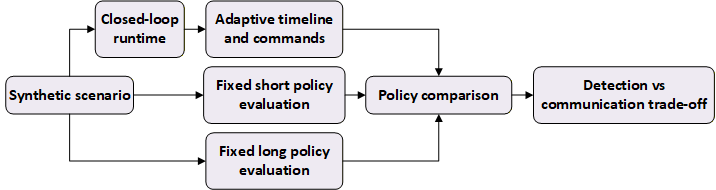
\includegraphics[width=\columnwidth]{fig/experimental_methodology2.png}
    \caption{Workflow of the comparative evaluation of the proposed framework.}
    \label{fig:experimental_methodology}
\end{figure}

\section{Results and Discussion}
\label{sec:Results_Discussion}
\subsection{Evidence of Closed-Loop Digital-Twin Execution}
In the reference execution reported in this work (the \textit{intermittent\_evening} scenario, seven days at native 5-minute resolution, fixed seed), the runtime traversed 2016 potential acquisition instances and observed 299 of them under the adaptive policy with \textit{weighted} fusion, distributed as 1751 instants in \textit{basal} mode, 168 in \textit{moderate} mode, and 97 in \textit{aggressive} mode, a distribution consistent with the 12:4:1 emission ratio expected from the native-resolution correction of Section~\ref{subsec:native_resolution} once mode-dwell hysteresis is accounted for. In this same execution, 57 reconfiguration commands were issued and 18 transport events fell back from NB-IoT to BLE. This evidence is architectural and operational, not merely classificatory: it demonstrates that the \textit{ForensicTwin}, \textit{DecisionEngine}, \textit{PolicyOrchestrator}, \textit{MockTransport}, and \textit{MockForensicDevice} were exercised as coupled components of a closed-loop architecture in which the observation process itself is a consequence of the twin's own decisions.

\subsection{Supervised Baseline: Accuracy, Discrimination, and Feature Importance}
On the same reference scenario, the logistic-regression baseline (1411 training and 605 held-out test instants, chronological split) achieved accuracy $0.9917$, precision $0.9298$, recall $0.9815$, F1-score $0.9550$, and AUROC $0.9948$. These values are high but, unlike results obtained prior to the realism corrections of Section~\ref{subsec:synthetic_realism}, are no longer at or extremely near the theoretical ceiling of $1.0000$ across every non-degenerate scenario, which is consistent with the classification task no longer being an artifact of the data-generation process. Fig.~\ref{fig:roc_curves} shows the corresponding ROC curve. A two-hidden-layer MLP trained on the same split achieved accuracy $0.9868$, precision $0.9600$, recall $0.8889$, F1-score $0.9231$, and AUROC $0.9981$; the additional model capacity did not translate into a higher F1-score in this scenario, indicating that the logistic-regression baseline is not capacity-limited on the engineered feature set.

\begin{figure}[!ht]
    \centering
    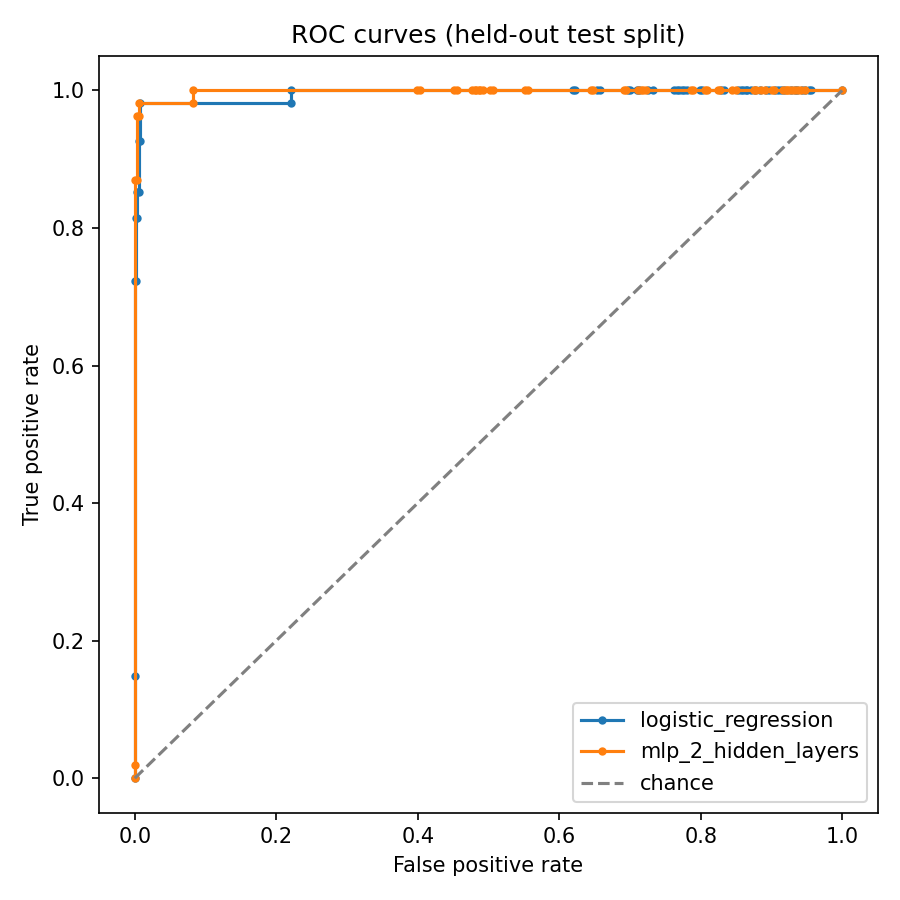
\includegraphics[width=\columnwidth]{fig/roc_curves.png}
    \caption{ROC curves for the logistic-regression and MLP baselines on the held-out test split of the reference scenario.}
    \label{fig:roc_curves}
\end{figure}

Permutation importance (F1-scoring, 20 repetitions) on the held-out split ranks \texttt{relative\_divergence} as the dominant feature (mean importance $0.783$), followed by \texttt{alarm\_score} ($0.145$) and \texttt{slot\_recurrence} ($0.074$); the five remaining features each contribute less than $0.02$ of mean importance. Standardized logistic-regression coefficients follow the same ranking (\texttt{relative\_divergence}: $6.84$; \texttt{alarm\_score}: $2.03$; \texttt{slot\_recurrence}: $0.73$). This confirms that electrical divergence remains, as expected, the primary detection signal, but with a measurable and non-deterministic contribution rather than a one-to-one encoding of the label, and that the alarm and temporal-recurrence features contribute genuine secondary evidence rather than a redundant restatement of the same signal.

\subsection{Aggregate Performance Against the True Dense-Monitoring Ceiling}
\label{subsec:results_headline}
\begin{table}[ht]
\centering
\caption{Aggregate comparison across the seven-scenario campaign (mean values).}
\label{tab:agg_policy_results}
\scriptsize
\begin{tabular}{lcccc}
\hline
\textbf{Policy} & \textbf{Source/fusion} & \textbf{F1} & \textbf{Recall} & \textbf{Bytes} \\
\hline
\textit{fixed\_dense} & Supervised & 0.5545 & 0.5705 & 137{,}835 \\
\textit{fixed\_dense} & Rule-based & 0.5219 & 0.5467 & 137{,}835 \\
\textit{adaptive} & Decision / weighted & 0.5039 & 0.4727 & 40{,}646 \\
\textit{adaptive} & Supervised / weighted & 0.5024 & 0.4729 & 40{,}646 \\
\textit{adaptive} & Rule-based / weighted & 0.4805 & 0.4548 & 40{,}646 \\
\textit{fixed\_short} & Supervised & 0.2699 & 0.1814 & 47{,}621 \\
\textit{fixed\_short} & Rule-based & 0.2550 & 0.1735 & 47{,}621 \\
\textit{fixed\_long} & Supervised & 0.0822 & 0.0447 & 17{,}514 \\
\textit{fixed\_long} & Rule-based & 0.0784 & 0.0427 & 17{,}514 \\
\hline
\end{tabular}
\end{table}

Table~\ref{tab:agg_policy_results} reports the aggregate comparison across the full seven-scenario campaign, evaluated as described in Section~\ref{sec:experimental_campaign}. The \textit{fixed\_dense} policy, reporting at the native 5-minute resolution, is the correct empirical ceiling for "what would detection performance be under the densest possible monitoring," and achieves a mean F1-score of $0.5545$ (supervised source) at a mean communication cost of $137{,}835$ bytes. The adaptive policy with \textit{weighted} fusion achieves a mean F1-score of $0.5039$ (decision probability) at $40{,}646$ bytes, retaining approximately $90.9\%$ of the dense-monitoring F1-score and $82.9\%$ of its recall while transmitting only approximately $29.5\%$ of the communication volume, a reduction of about $70.5\%$. This result holds consistently across probability sources: evaluating the same adaptive schedule under the supervised probability instead of the fused decision probability yields an essentially identical F1-score ($0.5024$) at the same communication cost, confirming that the benefit stems from the observation schedule itself rather than from a favorable choice of detection signal for one policy and not the others.

The mean values in Table~\ref{tab:agg_policy_results} should not be read as the detection quality attainable whenever theft is actually present, because three of the seven scenarios (\textit{normal}, \textit{disturbance\_without\_theft}, and \textit{degraded\_link\_no\_theft}) contain no theft instants by construction and therefore contribute a defined precision/recall/F1-score of exactly zero to the arithmetic mean, following the standard convention for an undefined ratio with no positive instances. Table~\ref{tab:scenario_breakdown} makes this explicit at the scenario level for both the \textit{fixed\_dense} ceiling and the \textit{adaptive} (weighted) policy. Restricting the mean to only the four scenarios that contain theft (\textit{persistent\_theft}, \textit{peak\_theft}, \textit{night\_theft}, and \textit{intermittent\_evening}) raises the \textit{fixed\_dense} figures to a mean F1-score of $0.9703$ and a mean recall of $0.9984$, consistent with the high area under the ROC curve reported in Fig.~\ref{fig:roc_curves}, and raises the \textit{adaptive} figures to a mean F1-score of $0.8819$ and a mean recall of $0.8272$. Notably, the \emph{retention ratio} between the adaptive policy and the dense ceiling, which is the quantity underlying the headline claim of this paper, is essentially unchanged by this restriction ($90.9\%$ of F1-score and $82.9\%$ of recall in both the seven-scenario and the four-scenario computation): because the three theft-free scenarios contribute an identical zero to both policies' means, they cancel out of the ratio algebraically and cannot, by construction, be inflating or deflating the reported retention percentage. The seven-scenario mean is nonetheless reported as the headline figure throughout this section because it also credits a policy for correctly producing zero false alerts on legitimate and degraded-link traffic, which is itself an operationally relevant outcome for a deployed system, not only a statistical artifact.

\begin{table*}[!ht]
\centering
\caption{Scenario-level detection performance and communication cost for the dense-monitoring ceiling and the adaptive policy.}
\label{tab:scenario_breakdown}
\begin{tabular}{lccccccc}
\hline
& & \multicolumn{3}{c}{\textit{fixed\_dense} (supervised)} & \multicolumn{3}{c}{\textit{adaptive} (weighted)} \\
\textbf{Scenario} & \textbf{Contains theft} & \textbf{F1} & \textbf{Recall} & \textbf{Bytes} & \textbf{F1} & \textbf{Recall} & \textbf{Bytes} \\
\hline
\textit{normal} & No & 0.0000 & 0.0000 & 135{,}452 & 0.0000 & 0.0000 & 17{,}736 \\
\textit{persistent\_theft} & Yes & 1.0000 & 1.0000 & 135{,}332 & 1.0000 & 1.0000 & 135{,}332 \\
\textit{peak\_theft} & Yes & 0.9264 & 0.9958 & 134{,}952 & 0.9159 & 0.8625 & 30{,}324 \\
\textit{night\_theft} & Yes & 0.9976 & 0.9976 & 135{,}152 & 0.9928 & 0.9881 & 41{,}884 \\
\textit{intermittent\_evening} & Yes & 0.9572 & 1.0000 & 135{,}212 & 0.6189 & 0.4581 & 25{,}204 \\
\textit{disturbance\_without\_theft} & No & 0.0000 & 0.0000 & 135{,}352 & 0.0000 & 0.0000 & 17{,}736 \\
\textit{degraded\_link\_no\_theft} & No & 0.0000 & 0.0000 & 153{,}396 & 0.0000 & 0.0000 & 16{,}304 \\
\hline
Mean, all 7 scenarios & --- & 0.5545 & 0.5705 & 137{,}835 & 0.5039 & 0.4727 & 40{,}646 \\
Mean, 4 theft-bearing scenarios & --- & 0.9703 & 0.9984 & 135{,}162 & 0.8819 & 0.8272 & 58{,}186 \\
\hline
\end{tabular}
\end{table*}

The scenario-level breakdown also identifies where the adaptive policy loses the most ground relative to the ceiling: in \textit{intermittent\_evening}, the campaign's most temporally erratic scenario (Section~\ref{subsec:synthetic_realism}), the adaptive policy's F1-score falls to $0.6189$ (recall $0.4581$), against $0.9572$ (recall $1.0000$) for \textit{fixed\_dense}, because the twin cannot always react in time to theft windows that activate unpredictably within a given evening. In \textit{peak\_theft} and \textit{night\_theft}, whose theft windows are temporally concentrated and therefore easier to anticipate once the twin has densified observation, the adaptive policy remains within about half a percentage point to about one percentage point of F1-score of the ceiling ($0.9928$ versus $0.9976$, and $0.9159$ versus $0.9264$, respectively) while using between $69\%$ and $78\%$ fewer bytes. This indicates that the aggregate retention figure reported above is not uniform across fraud behaviors, and that the adaptive policy's relative advantage is largest for temporally structured theft and smallest for highly erratic, short-notice theft.

The comparison against \textit{fixed\_short}, an intermediate 15-minute fixed cadence, is at least as informative: \textit{fixed\_short} is dominated by the adaptive policy in both dimensions simultaneously (F1-score $0.2699$ at a higher cost of $47{,}621$ bytes, versus F1-score $0.5039$ at $40{,}646$ bytes for the adaptive policy). This occurs because, once the native resolution was corrected (Section~\ref{subsec:native_resolution}), a fixed 15-minute cadence under-samples relative to the intermittent, short-lived fraud events represented in the campaign, while still incurring more communication cost than a policy that concentrates its (denser) sampling on the periods of elevated risk. The \textit{fixed\_long} policy, at the lowest cost ($17{,}514$ bytes), exhibits severe under-observation (F1-score $0.0822$, recall $0.0447$), confirming that permanently sparse monitoring is not a viable substitute for either dense or adaptive observation in this setting.

\subsection{Fusion-Strategy Ablation}
\label{subsec:results_fusion_ablation}
\begin{table}[ht]
\centering
\caption{Aggregate comparison of adaptive fusion strategies (mean, decision probability).}
\label{tab:agg_fusion_results}
\scriptsize
\begin{tabular}{lccc}
\hline
\textbf{Strategy} & \textbf{F1} & \textbf{Recall} & \textbf{Bytes} \\
\hline
\textit{weighted} & 0.5039 & 0.4727 & 40{,}646 \\
\textit{conservative\_max} & 0.4828 & 0.4694 & 41{,}105 \\
\textit{context\_aware} & 0.4714 & 0.4169 & 37{,}622 \\
\hline
\end{tabular}
\end{table}

Table~\ref{tab:agg_fusion_results} reports the aggregate comparison of the three fusion strategies. The \textit{weighted} strategy achieves the best mean F1-score. \textit{conservative\_max} is dominated by \textit{weighted} in both dimensions (lower F1-score at higher communication cost), confirming that inheriting the maximum of the two evidence sources over-amplifies isolated evidence into unnecessary densification without a corresponding detection benefit. \textit{context\_aware} trades approximately $6.4\%$ of the mean F1-score for an approximately $7.4\%$ reduction in communication cost relative to \textit{weighted}, which is a genuine, interpretable trade-off rather than a strict dominance in either direction; this indicates that the added semantic sophistication of context-dependent weighting did not, in this campaign, translate into a Pareto improvement over the simpler weighted combination, and that further refinement of the context-switching rules (Section~\ref{subsec:fusao}) would need to specifically target detection performance, not only cost, to outperform the weighted baseline outright.

\subsection{Critical-Slot Metric: Binary and Relaxed}
The binary critical-slot-hit metric is $0.5714$ (mean fraction of scenarios hit) for the adaptive policy and as low as $0.2857$ for \textit{fixed\_dense} under the rule-based source, despite the latter having a higher raw F1-score in that configuration; the relaxed score of Eq.~\eqref{eq:relaxed_critical_slot} resolves this apparent inconsistency, reporting $0.9496$ for the adaptive policy and $0.5394$ for \textit{fixed\_dense} (rule-based), which indicates that even the "misses" recorded by the binary metric were, on average, temporally close to the true busiest theft hour for the adaptive policy but more temporally dispersed for \textit{fixed\_dense} under the rule-based source. This confirms the value of reporting both metrics together, as recommended by the temporal-tolerance evaluation literature \cite{b36,b37}: the binary metric flags whether the policy achieved exact temporal precision, while the relaxed metric quantifies how operationally close a non-exact result still was.

\subsection{Communication-Cost Trade-off Resolution}
\label{subsec:results_pareto}
The grid search of Section~\ref{subsec:pareto} evaluated 60 configurations of $(\alpha, \tau_{\text{moderate}}, \tau_{\text{high}})$ on three representative scenarios, of which 30 aggregate configurations are Pareto-optimal in the $(D, C)$ plane. Fig.~\ref{fig:pareto_frontier} shows the resulting frontier. The configuration used elsewhere in this paper ($\alpha = 0.6$, $\tau_{\text{moderate}} = 0.30$, $\tau_{\text{high}} = 0.60$) achieves F1-score $0.869$ at a mean cost of $30{,}635$ bytes on this three-scenario subset; it lies close to, but not exactly on, the empirical frontier, whose nearest point at comparable cost ($\tau_{\text{high}} = 0.50$, all else equal) achieves F1-score $0.878$ at $30{,}751$ bytes, a difference of about one percentage point of F1-score at essentially the same communication cost. This is reported as an honest empirical characterization of the operating point actually used, rather than as a retroactive re-tuning of production defaults based on a three-scenario grid: the frontier is offered as a decision-support artifact for selecting an operating point according to the utility's own $\lambda_1/\lambda_2$ preference, consistent with the framing of Section~\ref{sec:system_model}.

\begin{figure}[!ht]
    \centering
    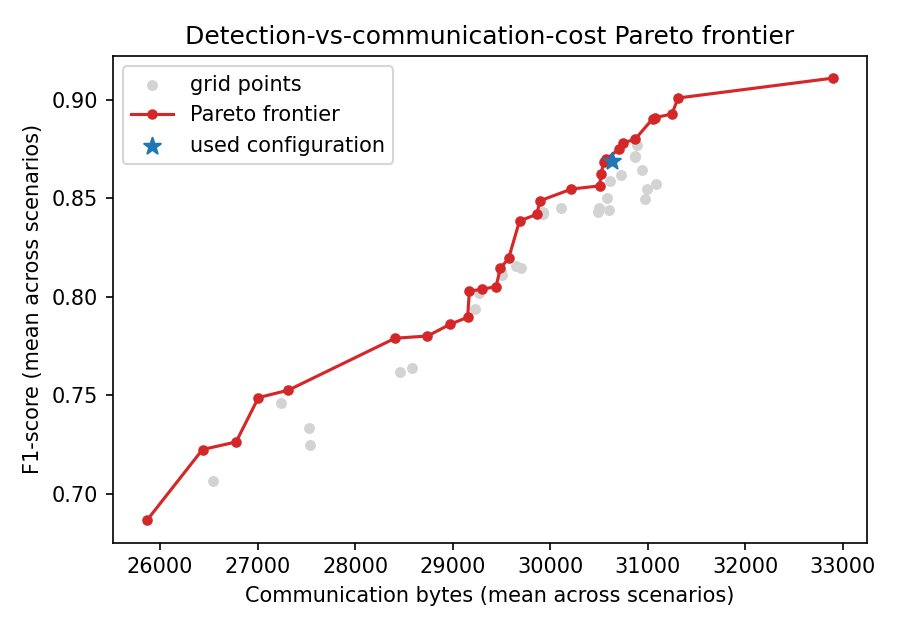
\includegraphics[width=\columnwidth]{fig/policy_pareto_frontier.png}
    \caption{Empirical Pareto frontier between detection (F1-score) and communication cost, obtained by grid search over the fusion weight and hysteresis thresholds. The star marks the configuration used elsewhere in this paper.}
    \label{fig:pareto_frontier}
\end{figure}

\subsection{Computational Complexity and Scalability}
\label{subsec:results_scalability}
Fig.~\ref{fig:scalability} reports the wall-clock time per twin and the peak memory usage as the number of sequentially processed twins grows from 1 to 100, each replaying the same 2016-event trace. The per-twin cost is essentially constant, ranging from $0.999$ s (single twin) to $1.051$ s (100 twins), a drift ratio of $1.05\times$ across two orders of magnitude of fleet size, and peak memory remains within $9.85$-$10.34$ MB throughout, confirming the $O(N \cdot T)$ worst-case, embarrassingly-parallel scaling argued analytically in Section~\ref{subsec:complexity}. This result was only obtained after correcting the $O(T^2)$ billing-meter lookup identified during the development of this benchmark (Section~\ref{subsec:complexity}); prior to that correction, per-twin cost grew with the length of the event trace, which is consistent with, and a useful illustration of, the general risk that an unindexed per-event lookup against a growing reference table can silently convert an intended linear pipeline into a quadratic one.

\begin{figure}[!ht]
    \centering
    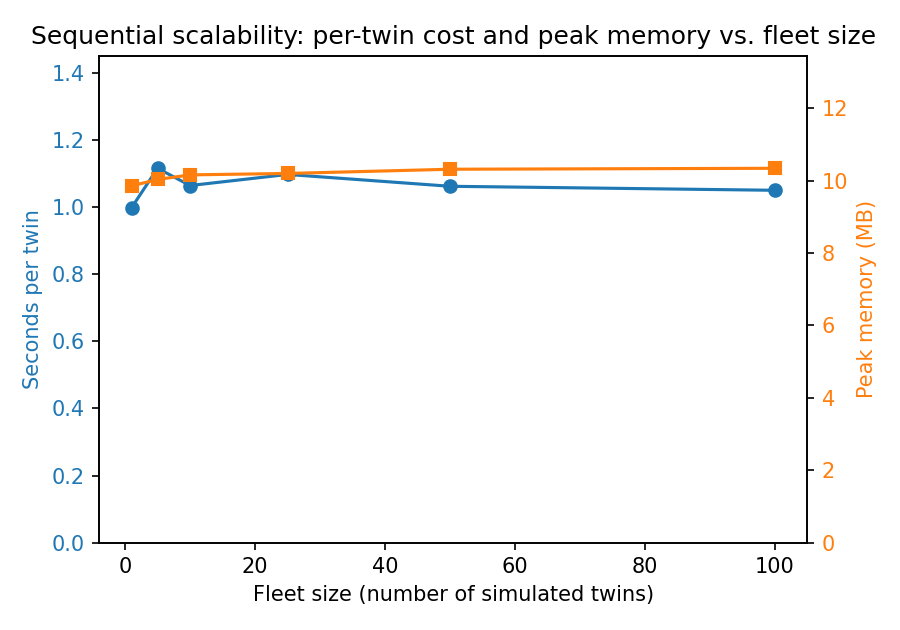
\includegraphics[width=\columnwidth]{fig/scalability_benchmark.png}
    \caption{Sequential wall-clock cost per twin and peak memory usage as a function of fleet size.}
    \label{fig:scalability}
\end{figure}

\subsection{Strengths of the Implementation and Experimental Evidence}
The results reinforce five main strengths of the implementation. First, the framework materializes a closed-loop digital twin, with the physical-versus-software synchronization scope stated explicitly (Section~\ref{subsec:twin_criteria}), rather than a static classification pipeline. Second, the adaptive policy substantially reduces communication cost while retaining most of the detection performance of the true dense-monitoring ceiling, a comparison that is now measured against the correct reference point rather than an intermediate fixed cadence. Third, the classification problem is no longer an artifact of the data-generation process, as evidenced by non-perfect, heterogeneous detection metrics across scenarios and by an explicit accounting of which scenarios are degenerate by construction. Fourth, the detection-versus-cost trade-off and the computational scalability of the approach are characterized empirically rather than asserted. Fifth, the traceability architecture (state history, decisions, commands, transport deliveries, and manifests) connects every reported number in this section to a specific, regenerable artifact, and the underlying source code and scripts are available from the corresponding author upon request (see Data Availability, below).

\subsection{Threats to Validity and Limitations}
\label{subsec:limitations}
Several limitations constrain the scope of the conclusions that can be drawn from this study, and are stated explicitly rather than left implicit. First, and most importantly, validation relies entirely on synthetic scenarios; although a distribution utility partner already collects field forensic-telemetry data of the kind targeted by this framework, that data is presently subject to an ongoing forensic and legal evaluation process to support corrective action against customers with indications of fraud, and cannot yet be disclosed for research publication. Consequently, this study validates the framework's internal coherence and its behavior under controlled, heterogeneous synthetic conditions, and field-data validation is identified as the primary direction for future work rather than as an omission. Second, the physical bidirectional synchronization criterion of Section~\ref{subsec:twin_criteria} is satisfied only in a local, reproducible simulation; end-to-end integration with a deployed NB-IoT/BLE radio link remains future work, and the communication-cost model, while grounded in reported measurement studies (Section~\ref{subsec:network_cost}), is not itself a field measurement. Third, the Pareto-frontier analysis of Section~\ref{subsec:pareto} restricts the search to a three-parameter hysteresis-policy family evaluated on three scenarios for computational tractability; it resolves the trade-off empirically within that family but does not constitute a proof of global optimality over the full action-sequence space of Section~\ref{sec:system_model}, and a sequential decision-making formulation (e.g., a partially observable Markov decision process solved by reinforcement learning, as has been explored for related adaptive-sampling and theft-detection problems \cite{b38}) is a natural extension for removing this restriction. Fourth, the \textit{context\_aware} fusion strategy did not outperform the simpler \textit{weighted} strategy in this campaign (Section~\ref{subsec:results_fusion_ablation}); this is reported as a negative result rather than omitted, and indicates that the value of contextual fusion depends on further refinement of its switching rules. Fifth, the computational-scalability benchmark of Section~\ref{subsec:results_scalability} measures a single-process, sequential execution as a conservative worst case; a production deployment across many devices would naturally be parallelized, which would only improve on the reported wall-clock figures.

\section{Conclusion}
\label{sec:Conclusion}
This work demonstrated that an application-oriented digital twin can use contextual theft-risk estimates to adapt the observation window of NB-IoT forensic telemetry, formalizing detection capability and communication cost as explicit functions of the twin's observational state and selected action, and resolving their trade-off empirically through a Pareto-frontier analysis rather than through unjustified fixed weights. Across a seven-scenario experimental campaign built with heterogeneous fraud severities, independent measurement and communication noise, and a native acquisition resolution fine enough to make every observation mode operationally distinguishable, the adaptive policy retained approximately 91\% of the F1-score and 83\% of the recall of the true dense-monitoring ceiling while transmitting approximately 30\% of the communication volume, and dominated an intermediate fixed-cadence baseline in both detection and cost simultaneously. A communication-cost model grounded in reported NB-IoT quality-of-service measurements, a feature-importance and alternative-model analysis, a relaxed temporal-tolerance metric, and an empirically verified linear computational-scalability result complement these findings.

Beyond these numerical results, the study demonstrates a conceptual shift from static classification to adaptive observation control, with the digital twin operating as an explicit-state, closed-loop decision layer whose criteria for that label are stated and checked individually rather than asserted. The framework's physical bidirectional synchronization is, at present, closed only in a local, reproducible simulation, and its detection-versus-cost trade-off is resolved within a restricted, interpretable policy family; field-data validation, end-to-end NB-IoT/BLE integration, and a sequential decision-making formulation of the observation policy are identified as the primary directions for future work. Contextual risk-driven adaptation is shown to be a technically coherent and quantitatively characterized strategy for forensic telemetry in communication-constrained smart-metering environments.

\section*{Data Availability}
This paper repeatedly describes the underlying prototype as reproducible, on the basis of its deterministic synthetic-data generation, its explicit twin-state and command-plan traceability artifacts (Section~\ref{sec:Materials_Methods}), and the fact that every table and figure in Section~\ref{sec:Results_Discussion} is produced by a documented, script-driven pipeline rather than by manual computation. At the time of this submission, however, no public code repository or dataset deposit had yet been established, and this is disclosed explicitly rather than left for a reader to infer. The full source code, including the digital-twin components (\textit{ForensicTwin}, \textit{DecisionEngine}, \textit{PolicyOrchestrator}), the synthetic-data generator, the mock device/transport/billing-meter simulators, and the analysis scripts used for the Pareto-frontier and scalability results, together with the synthetic datasets and generated artifacts underlying every reported number, is available from the corresponding author upon reasonable request.

\section*{Acknowledgment}
This work was supported in part by the Coordenação de Aperfeiçoamento de Pessoal de Nível Superior (CAPES), Brazil, Finance Code 001, and by the Programa de Excelência Acadêmica (PROEX). The authors also acknowledge the Núcleo de Estudos e Pesquisas do Norte e Nordeste (NEPEN), Instituto Constanta de Inovação (ICI), and EDP South America for providing the infrastructure and material resources essential to the execution of this research, conducted under ANEEL R\&D project PD-00391-0054/25. The authors acknowledge the limited use of AI-based tools for language refinement and auxiliary literature exploration during manuscript preparation.

\begin{thebibliography}{00}

\bibitem{b1} Jeyaraj, P., Nadar, E., Kathiresan, A., \& Asokan, S. (2020). Smart grid security enhancement by detection and classification of non‐technical losses employing deep learning algorithm. International Transactions on Electrical Energy Systems, 30. https://doi.org/10.1002/2050-7038.12521.

\bibitem{b2} Hasan, M., Toma, R., Nahid, A., Islam, M., \& Kim, J. (2019). Electricity Theft Detection in Smart Grid Systems: A CNN-LSTM Based Approach. Energies. https://doi.org/10.3390/en12173310.

\bibitem{b3} Gul, H., Javaid, N., Ullah, I., Qamar, A., Afzal, M., \& Joshi, G. (2020). Detection of Non-Technical Losses Using SOSTLink and Bidirectional Gated Recurrent Unit to Secure Smart Meters. Applied Sciences. https://doi.org/10.3390/app10093151.

\bibitem{b4} Kawoosa, A., Prashar, D., Faheem, M., Jha, N., \& Khan, A. (2023). Using machine learning ensemble method for detection of energy theft in smart meters. IET Generation, Transmission \& Distribution. https://doi.org/10.1049/gtd2.12997.

\bibitem{b5} Hashim, M., Khan, L., Javaid, N., Ullah, Z., \& Javed, A. (2024). Stacked machine learning models for non-technical loss detection in smart grid: A comparative analysis. Energy Reports. https://doi.org/10.1016/j.egyr.2024.06.015.

\bibitem{b6} Massarani, A., Badr, M., Baza, M., Alshahrani, H., \& Alshehri, A. (2025). Efficient and Accurate Zero-Day Electricity Theft Detection from Smart Meter Sensor Data Using Prototype and Ensemble Learning. Sensors (Basel, Switzerland), 25. https://doi.org/10.3390/s25134111.

\bibitem{b7} Gunduz, M., \& Daş, R. (2024). Smart Grid Security: An Effective Hybrid CNN-Based Approach for Detecting Energy Theft Using Consumption Patterns. Sensors (Basel, Switzerland), 24. https://doi.org/10.3390/s24041148.

\bibitem{b8} Ali, A., Khan, L., Javaid, N., Bouk, S., Aldegheishem, A., \& Alrajeh, N. (2023). Mitigating anomalous electricity consumption in smart cities using an AI‐based stacked‐generalization technique. IET Renewable Power Generation. https://doi.org/10.1049/rpg2.12785.

\bibitem{b9} Mu, T., Yu, Y., Feng, G., Luo, H., \& Yang, H. (2023). Detecting anomalous electricity consumption with transformer and synthesized anomalies. PeerJ Computer Science, 9. https://doi.org/10.7717/peerj-cs.1721.

\bibitem{b10} Žarković, M., \& Dobrić, G. (2024). Artificial Intelligence for Energy Theft Detection in Distribution Networks. Energies. https://doi.org/10.3390/en17071580.

\bibitem{b11} Vasantrao, J., \& Patel, C. (2025). AT\&C and non-technical loss reduction in smart grid using smart metering with AI techniques. The Scientific Temper. https://doi.org/10.58414/scientifictemper.2025.16.8.06.

\bibitem{b12} Blazakis, K., Schetakis, N., Badr, M., Aghamalyan, D., Stavrakakis, K., \& Stavrakakis, G. (2025). Power Theft Detection in Smart Grids Using Quantum Machine Learning. IEEE Access, 13, 61511-61525. https://doi.org/10.1109/access.2025.3558143.

\bibitem{b13} Maamar, A., \& Benahmed, K. (2019). A Hybrid Model for Anomalies Detection in AMI System Combining K-means Clustering and Deep Neural Network. Computers, Materials \& Continua. https://doi.org/10.32604/cmc.2019.06497.

\bibitem{b14} Kawoosa, A., Prashar, D., Raman, A., Bijalwan, A., Haq, M., Aleisa, M., \& Alenizi, A. (2024). Improving Electricity Theft Detection Using Electricity Information Collection System and Customers’ Consumption Patterns. Energy Exploration \& Exploitation, 42, 1684 - 1714. https://doi.org/10.1177/01445987241255394.

\bibitem{b15} Callcut, M., Agliozzo, J., Varga, L., \& McMillan, L. (2021). Digital Twins in Civil Infrastructure Systems. Sustainability. https://doi.org/10.3390/su132011549.

\bibitem{b16} Dihan, M., Akash, A., Tasneem, Z., Das, P., Das, S., Islam, M., Islam, M., Badal, F., Ali, M., Ahmed, M., Abhi, S., Sarker, S., \& Hasan, M. (2024). Digital twin: Data exploration, architecture, implementation and future. Heliyon, 10. https://doi.org/10.1016/j.heliyon.2024.e26503.

\bibitem{b17} Somma, A., Amalfitano, D., De Benedictis, A., \& Pelliccione, P. (2025). TwinArch: A Digital Twin Reference Architecture. ArXiv, abs/2504.07530. https://doi.org/10.1016/j.jss.2025.112613.

\bibitem{b18} Elsisi, M., Mahmoud, K., Lehtonen, M., \& Darwish, M. (2021). Reliable Industry 4.0 Based on Machine Learning and IoT for Analyzing, Monitoring, and Securing Smart Meters. Sensors (Basel, Switzerland), 21. https://doi.org/10.3390/s21020487.

\bibitem{b19} Habib, M., Shoukat, M., Irfan, M., Zubair, M., Ahmed, S., Raza, M., Ali, T., \& Sarwar, A. (2023). Smart Meter Development Using Digital Twin Technology for Green Energy Distribution Optimization. European Journal of Theoretical and Applied Sciences. https://doi.org/10.59324/ejtas.2023.1(3).20.

\bibitem{b20} Irfan, M., Niaz, A., Habib, M., Shoukat, M., Atta, S., \& Ali, A. (2023). Digital Twin Concept, Method and Technical Framework for Smart Meters. European Journal of Theoretical and Applied Sciences. https://doi.org/10.59324/ejtas.2023.1(3).10.

\bibitem{b21} Han, F., Du, F., Jiao, S., \& Zou, K. (2024). Predictive Analysis of a Building’s Power Consumption Based on Digital Twin Platforms. Energies. https://doi.org/10.3390/en17153692.

\bibitem{b22} Zaheen, M., Arshad, R., Ain, A., Sarwar, A., \& Khan, M. (2025). Digital Twin-Based Smart Metering Framework with Real-Time Monitoring via Microsoft Azure IoT. 2025 20th International Conference on Emerging Technologies (ICET), 1-7. https://doi.org/10.1109/icet66147.2025.11321353.

\bibitem{b23} Mahmoodian, M., Shahrivar, F., Setunge, S., \& Mazaheri, S. (2022). Development of Digital Twin for Intelligent Maintenance of Civil Infrastructure. Sustainability. https://doi.org/10.3390/su14148664.

\bibitem{b24} Almasan, P., Galmés, M., Paillissé, J., Suárez-Varela, J., Perino, D., López, D., Perales, A., Harvey, P., Ciavaglia, L., Wong, L., Ram, V., Xiao, S., Shi, X., Cheng, X., Cabellos-Aparicio, A., \& Barlet-Ros, P. (2022). Digital Twin Network: Opportunities and Challenges. ArXiv, abs/2201.01144.

\bibitem{b25} Liu, H., Wen, W., Gou, W., Lu, X., H., Zhu, L., Zhang, M., Wu, S., \& Guo, X. (2025). Research on Intelligent Control Technology for a Rail-Based High-Throughput Crop Phenotypic Platform Based on Digital Twins. Agriculture. https://doi.org/10.3390/agriculture15111217.

\bibitem{b26} Qaddoori, S., \& Ali, Q. (2023). An embedded and intelligent anomaly power consumption detection system based on smart metering. IET Wirel. Sens. Syst., 13, 75-90. https://doi.org/10.1049/wss2.12054.

\bibitem{b27} Raeiszadeh, M., Ebrahimzadeh, A., Glitho, R., Eker, J., \& Mini, R. (2024). Real-Time Adaptive Anomaly Detection in Industrial IoT Environments. IEEE Transactions on Network and Service Management, 21, 6839-6856. https://doi.org/10.1109/tnsm.2024.3447532.

\bibitem{b28} Sayed, A., Ruiz, M., Harb, H., \& Velasco, L. (2023). Deep Learning-Based Adaptive Compression and Anomaly Detection for Smart B5G Use Cases Operation. Sensors (Basel, Switzerland), 23. https://doi.org/10.3390/s23021043.

\bibitem{b29} Al-Sammak, K., Al-Gburi, S., Marghescu, I., Drãgulinescu, A., Marghescu, C., Martian, A., Al-Sammak, N., Suciu, G., \& Alheeti, K. (2025). Optimizing IoT Energy Efficiency: Real-Time Adaptive Algorithms for Smart Meters with LoRaWAN and NB-IoT. Energies. https://doi.org/10.3390/en18040987.

\bibitem{b30} Fan, X., Zhou, C., Sun, Y., Du, J., \& Zhao, Y. (2019). Research on Remote Meter Reading Scheme and IoT Smart Energy Meter Based on NB-IoT Technology. Journal of Physics: Conference Series, 1187. https://doi.org/10.1088/1742-6596/1187/2/022064.

\bibitem{b31} Maduranga, M., \& Wijerathna, A. (2022). NB-IoT based Status Measurement System for 33kV Power Distribution Networks in Smart Grids. International Journal of Engineering and Manufacturing. https://doi.org/10.5815/ijem.2022.04.04.

\bibitem{b32} Sultania, A. K., \& Famaey, J. (2020). Real-Time Demand Response Using NB-IoT. IEEE Internet of Things Journal, 8(9), 7273-7285. https://doi.org/10.1109/JIOT.2020.3038767.

\bibitem{b33} Stusek, M., Masek, P., Sabol, T., Kral, J., Kolackova, K., Zeman, K., Mikhaylov, K., \& Hosek, J. (2023). Exploiting NB-IoT Network Performance and Capacity for Smart-Metering Use-Cases. 2023 15th International Congress on Ultra Modern Telecommunications and Control Systems and Workshops (ICUMT).

\bibitem{b34} Matz, A. P., Fernández-Prieto, J. A., Cañada-Bago, J., \& Birkel, U. (2020). A Systematic Analysis of Narrowband IoT Quality of Service. Sensors (Basel, Switzerland), 20. https://doi.org/10.3390/s20061636.

\bibitem{b35} Sultania, A. K., \& Famaey, J. (2021). Optimizing the Energy-Latency Tradeoff in NB-IoT With PSM and eDRX. IEEE Internet of Things Journal, 8(23), 16729-16746. https://doi.org/10.1109/JIOT.2021.3075463.

\bibitem{b36} Salles, R., Belloze, K., Porto, F., Gonzalez, P., \& Ogasawara, E. (2023). SoftED: Metrics for Soft Evaluation of Time Series Event Detection. arXiv preprint, arXiv:2304.00439.

\bibitem{b37} Scharwächter, E., \& Müller, E. (2020). Statistical Evaluation of Anomaly Detectors for Sequences. arXiv preprint, arXiv:2010.15472.

\bibitem{b38} El-Toukhy, A. T., Mahmoud, M. M. E. A., Songhorabadi, M., Alasmary, W., \& Sherif, A. B. T. (2023). Electricity Theft Detection Using Deep Reinforcement Learning in Smart Power Grids. IEEE Access, 11, 59558-59575. https://doi.org/10.1109/ACCESS.2023.3285055.

\end{thebibliography}

\EOD

\end{document}
